
\chapter{Model-Based Clustering}
\label{chp:pmclust}

\section{Introduction}

Model-based clustering~\index{Model-Based Clustering}
is an unsupervised learning technique~\index{unsupervised learning}
and mainly based on finite mixture models to fit the data, cluster the data,
and draw inference from the data~\citep{Fraley2002,Melnykov2010}. The major application of
model-based clustering focuses on Gaussian mixture models. For example,
$\bX_n$ is a random $p$-dimensional observation from
the Gaussian mixture model~\index{Gaussian mixture model}
with $K$ components, which has density
\begin{equation}
f(\bX_n; \bTheta) = \sum_{k = 1}^K \eta_k \phi_p(\bX_n; \bmu_k, \bSigma_k)
\label{eqn:gaussian_mixture}
\end{equation}
where $\phi_p(\cdot;\cdot,\cdot)$ is a $p$-dimensional Gaussian density,
$$
\bTheta = \{\eta_1, \eta_2, \ldots, \eta_{K-1},
\bmu_1, \bmu_2, \ldots, \bmu_K, \bSigma_1, \bSigma_2, \ldots, \bSigma_K\},
$$
is the parameter space,
$\eta_k$'s are mixing proportion, $\bmu_k$'s are the centers of the components, and
$\bSigma_k$'s are the dispersion of the components.

Suppose a data set $\bX = \{\bX_1, \bX_2, \ldots, \bX_N\}$ has
$N$ observations.  Then the log likelihood is
\begin{equation}
\log L(\bTheta; \bX) = \sum_{n = 1}^N \log f(\bX_n; \bTheta)
\label{eqn:gaussian_mixture_logl}
\end{equation}
where $f$ is as in Equation~(\ref{eqn:gaussian_mixture}).
Solving the problem of maximizing this log-likelihood is usually done by the expectation-maximization (EM)
algorithm~\citep{Dempster1977}.~\index{EM algorithm}
Assuming the EM algorithm converges, we let $\hat{\bTheta}$ be the
maximum likelihood estimator of Equation~(\ref{eqn:gaussian_mixture_logl}).
Then the maximum posterior probability
$$
\argmax_k
\frac{\hat{\eta}_k\phi_p(\bX_n; \hat{\bmu}_k, \hat{\bSigma}_k)
    }{f(\bX_n; \hat{\bTheta})}
$$
for $n = 1, 2, \ldots, N$
indicates the membership of the observations of the data set $\bX$.


The \pkg{mclust}~\citep{mclust}~\index{mclust} and
\pkg{EMCluster}~\citep{Chen2012EMClusterpackage}~\index{EMCluster} packages
are the two main \proglang{R} packages implementing the EM algorithm for the
model-based clustering.
The \pkg{mclust} package has several selections on different kinds of models one may fit, while \pkg{EMCluster} 
implements the most complicated model (dispersions are all unstructured)
in a more efficient way, using several initializations, and
semi-supervised learning.~\index{semi-supervised learning}
However, both assume small $N$ and tiny $p$, and only run in serial with
sufficient memory.

Note that the k-means algorithm~\citep{Forgy1965}~\index{k-means}
equivalently assumes
$\eta_1 = \eta_2 = \cdots = \eta_K \equiv 1/K$ and
$\bSigma_1 = \bSigma_2 = \cdots = \bSigma_K \equiv \bI$
in Equation~(\ref{eqn:gaussian_mixture}), where
$\bI$ is the identity matrix.
As such, the k-means algorithm is a restricted Gaussian mixture model, such that
it can be implemented with a simplified version of the EM algorithm.
However, due to its strict assumptions, the cluster results are almost always unrealistic, leaving the data scientist unable to draw meaningful inference from the data, and sometimes have unreasonably high classification errors.


\subsection{Parallel Model-Based Clustering}

The \pkg{pmclust}~\citep{Chen2012pmclustpackage}~\index{pmclust} package is an \proglang{R}
package for parallel model-based clustering based on Gaussian mixture models
with unstructured dispersions.  The package uses data parallelism to solve one very large clustering problem, rather than the embarrassingly parallel problem of fitting many independent models to dataset(s).  This approach is especially useful for large, distributed platforms, where the data will be distributed across nodes.  And of course it is worth nothing that the package does not merely perform a local clustering operation on the local data pieces; some \code{gather} and \code{reduce} operations are necessary at some stages of the distributed EM algorithm.

An expectation-gathering-maximization (EGM)
algorithm~\citep{Chen2013}~\index{EGM}
is established for minimizing communication and data movement between nodes.
There are four variants of EGM-like algorithms implemented in \pkg{pmclust}
including EM, AECM~\citep{Meng1997}~\index{AECM},
APECM~\citep{Chen2011}~\index{APECM}, and APECMa~\citep{Chen2013}~\index{APECMa}. The variants are trying to achieve
better convergence rates and less computing time than the original EM algorithm.
For completeness' sake, a simple k-means algorithm is also implemented in \pkg{pmclust}.

The \pkg{pmclust} package is the first
\proglang{pbdR} application, and the first
\proglang{R} package in SPMD to analyze distributed data in terabyte scale.
It was originally designed for analyzing Climate simulation outputs (CAM5),
as discussed in Section~\ref{sec:pbdNCDF4_introduction}, and
is a product for the project
``Visual Data Exploration and Analysis of Ultra-large Climate Data''
supported by U.S. DOE Office of Science.

The \pkg{pmclust} package initially depended on \pkg{Rmpi}, but
designed in SPMD approach rather than in the master/worker paradigm even before
\proglang{pbdR} existed.
Later, it migrated to use \pkg{pbdMPI}~\citep{Chen2012pbdMPIpackage}
because of performance issues with \pkg{Rmpi} on larger machines.
So, by default, the package assumes data are stored in
SPMD row-major matrix format.

Currently, the package also utilizes
\pkg{pbdSLAP}~\citep{Chen2012pbdSLAPpackage},
\pkg{pbdBASE}~\citep{Schmidt2012pbdBASEpackage}, and
\pkg{pbdDMAT}~\citep{Schmidt2012pbdDMATpackage}
to implement a subset of the above algorithms for data in the \code{ddmatrix} format.
Table~\ref{tab:pmclust_algorithm} lists the current implementations.
\begin{table}[h]
\centering
\caption[Parallel Mode-Based Clustering Algorithms in \pkg{pmclust}]{
Parallel Mode-Based Clustering Algorithms in \pkg{pmclust}}
\label{tab:pmclust_algorithm}
\begin{tabular}{ccc} \hline\hline
Algorithm & SPMD & \code{ddmatrix} \\ \hline
EM        & yes  & no              \\
AECM      & yes  & no              \\
APECM     & yes  & no              \\
APECMa    & yes  & no              \\
k-means   & yes  & yes             \\ \hline\hline
\multicolumn{3}{c}{
Based on \pkg{pmclust} version 0.1-4}
\end{tabular}
\end{table}


\section{An Example Using the {\it Iris} Dataset}

The \code{iris}~\citep{Fisher1936}~\index{iris} dataset is a famous dataset available in \proglang{R}
consisting of 50 iris flowers from each of three species of iris,
namely {\it Iris setosa}, {\it Iris versicolor}, and {\it Iris virginica}.
The dataset is tiny, even by today's standards, with only 150 rows and five columns.  The column variables consist of the
four features sepal length, sepal width, petal length, and petal width, as well as the
class of species.
We take the first four columns of \code{iris} to form the matrix $\bX$, 
where each row can be
classified in three groups by the true id (the fifth column of \code{iris})
for supervised learning,
or clustered in three groups by algorithms for unsupervised learning.
Note that the dimension of $\bX$ is $N = 150$ by $p = 4$.

Figure~\ref{fig:iris_pairs} shows the pair-wised scatter plot for all features
denoted on the diagonal, and classes are indicated by colors. Each panel
plots two features on x and y axes. It is clear
that \code{Petal.Length} can split three species in two groups. However,
one of the group is mixed with two species and can not be distinguished by
any one of these four features.
\begin{figure}[h!bt]
  \centering
  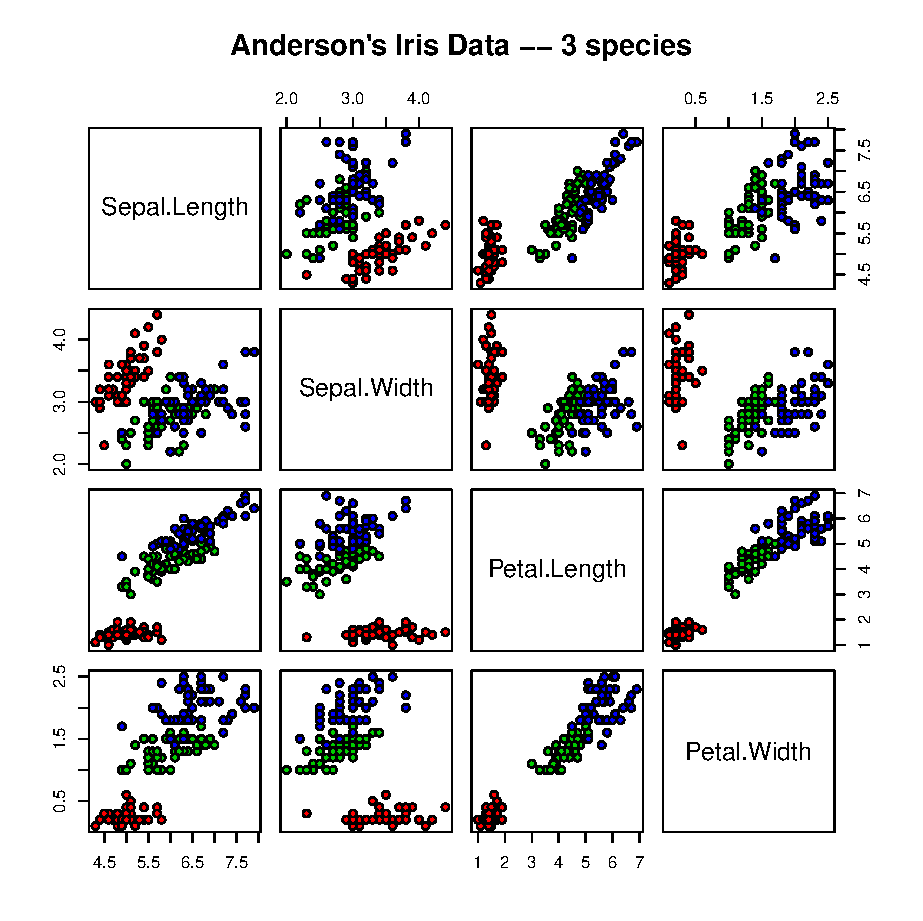
\includegraphics[width=6.5in]{pbdDEMO-include/pics/iris_pairs.pdf}
  \vspace{-1.5cm}
  \caption[Iris pair-wised scatter plot]{
    Iris pair-wised scatter plot. {\it Iris setosa} is in red,
    {\it Iris versicolor} is in green, and {\it Iris virginica} is in blue.
  }
  \label{fig:iris_pairs}
\end{figure}


From the supervised learning point view, the empirical estimation for
$\bTheta$ from data will be the best description for the data, assuming
the ``true model'' is a Gaussian mixture. The (serial) demo code \code{iris_overlap} in
\pkg{pbdDEMO} quickly suggests the overlap level of three
iris species. It can be obtained by executing:
\begin{Code}[title=R Code]
R> demo(iris_overlap, 'pbdDEMO', ask = F, echo = F)
\end{Code}
which utilizes the \code{overlap} function of \pkg{MixSim}~\citep{Melnykov2012}.
The output is:
\begin{CodeOutput}
R> (ret <- overlap(ETA, MU, S))
$OmegaMap
             [,1]         [,2]       [,3]
[1,] 1.000000e+00 7.201413e-08 0.00000000
[2,] 1.158418e-07 1.000000e+00 0.02302315
[3,] 0.000000e+00 2.629446e-02 1.00000000

$BarOmega
[1] 0.01643926

$MaxOmega
[1] 0.0493176

$rcMax
[1] 2 3

R> (levels(iris[, 5]))
[1] "setosa"     "versicolor" "virginica"
\end{CodeOutput}
The \code{OmegaMap} matrix is a map of pair-wise overlap of three species
where rows/columns 1, 2, and 3 are {\it Iris setosa}, {\it Iris versicolor}, and
{\it Iris virginica}, respectively.
The outputs also indicate that the averaged pair-wised overlap (\code{BarOmega})
is about $1.6\%$, and the maximum pair-wised overlap (\code{MaxOmega}) is
about $4.9\%$ among these three iris species. Also,
the maximum occurs at 2 ({\it Iris versicolor}) and 3 ({\it Iris virginica})
indicating these two species are partly inseparable given these four features.

From the unsupervised learning point view, such as model-based clustering,
we must pretend that we are blind to the true class ids, or said another way, we must
treat the fifth column of $\bX$ as unobserved.  We can then use the four
features to form the model and cluster the data, then go back and compare our unsupervised learning
results to the true values.

Note that
{\it Iris versicolor} and {\it Iris virginica} are partly inseparable,
so misclassification can happen at the overlap region.
We validate the results by comparing the clustering ids
to the true class ids using adjusted Rand index~\citep{Hubert1985}.
The adjusted Rand index takes values between -1 and 1, where 0 is a perfect
match. The function \code{RRand} in \pkg{MixSim}
also provides the adjusted Rand index.

The analysis in the unsupervised learning approach proceeds as follows:
\begin{enumerate}
\item decompose $\bX$ on its principal components,
\item project $\bX$ onto the first two principal components (those with largest variability),
\item fit a k-means model and a mbc model, and finally
\item visualize $\bX$ on the the plane formed by these new axes, labeling the entries of $\bX$ on this plot with the true ids, and the estimated ids from the clustering algorithms.
\end{enumerate}
This will be the general procedure whether in serial or parallel.  For example's sake, we will extend these steps 
to offer SPMD code and \code{ddmatrix} code to show the similarity of codes.

This example demonstrates that the \pkg{pmclust} package can generate perform analyses correctly, but is not
meant to be a demonstration of its scalability prowess.  The \code{iris} dataset is, by any reasonable definition, tiny.  Small datasets are generally not worth the trouble of developing parallelized analysis codes for, especially since all the extra overhead costs inherent to parallelism might dominate any theoretical performance gains.  Again, the merit of the example is to show off the syntax and accuracy on a single machine; however, \pkg{pmclust} scales up nicely to very large dataset running on supercomputers.



\subsection{{\it Iris} in Serial Code and Sample Outputs}

\subsubsection{Code}
The code here is fairly self-explanatory and well-documented besides, so no additional commentary is provided.

\textbf{Step 1:}  PCA\vspace{-.6cm}
\begin{lstlisting}[language=rr]
### Load data
X <- as.matrix(iris[, -5])         # Dimension 150 by 4
X.cid <- as.numeric(iris[, 5])     # True id

### Transformation and check
X.std <- scale(X)                  # Standardize
mu <- colMeans(X.std)              # Columns means are near 0
cov <- cov(X.std)                  # Diagonals are near 1
print(mu)
print(cov)

### SVD
X.svd <- svd(X.std)
\end{lstlisting}

\textbf{Step 2:}  Project onto the first two PC's\vspace{-.6cm}
\begin{lstlisting}[language=rr]
### Project on column space of singular vectors; three equivalent ways
A <- X.std %*% diag(X.svd$d)
B <- X.std %*% X.svd$v
C <- prcomp(X.std)$x               # A = B = C

X.prj <- C[, 1:2]                  # project onto first 2 PC's
\end{lstlisting}

\textbf{Step 3:}  Cluster\vspace{-.6cm}
\begin{lstlisting}[language=rr]
### Clustering
set.seed(1234)                     # Set overall seed
X.kms <- kmeans(X.std, 3)          # K-means
X.kms
X.kms.cid <- X.kms$cluster         # Classification

library(EMCluster)                 # Model-based clustering
X.mbc <- init.EM(X.std, 3)         # Initial by em-EM
X.mbc
X.mbc.cid <- X.mbc$class           # Classification


### Validation
# k-means adjusted Rand index
X.kms.adjR <- RRand(X.cid, X.kms.cid)$adjRand 
# MBC adjusted Rand index
X.mbc.adjR <- RRand(X.cid, X.mbc.cid)$adjRand  


### Swap classification id
X.kms.cid[X.kms.cid == 2] <- 4
X.kms.cid[X.kms.cid == 3] <- 2
X.kms.cid[X.kms.cid == 4] <- 3
\end{lstlisting}

\textbf{Step 4:}  Visualize\vspace{-.6cm}
\begin{lstlisting}[language=rr]
### Display on first 2 components
pdf("serial_plot.pdf")

par(mfrow = c(2, 2))
plot(X.prj, col = X.cid + 1, pch = X.cid,
     main = "iris (true)", xlab = "PC1", ylab = "PC2")
plot(X.prj, col = X.kms.cid + 1, pch = X.kms.cid,
     main = paste("iris (k-Means)", sprintf("%.4f", X.kms.adjR)),
     xlab = "PC1", ylab = "PC2")
plot(X.prj, col = X.mbc.cid + 1, pch = X.mbc.cid,
     main = paste("iris (Model-based)", sprintf("%.4f", X.mbc.adjR)),
     xlab = "PC1", ylab = "PC2")
accuracy <- c(X.kms.adjR, X.mbc.adjR)
names(accuracy) <- c("k-Means", "Model-based")
barplot(accuracy, main = "Clustering Accuracy")

dev.off()
\end{lstlisting}

\subsubsection{Sample Outputs}
Running this script should produce an ouput that looks something like the following:
\begin{Output}
 Sepal.Length   Sepal.Width  Petal.Length   Petal.Width 
-4.480675e-16  2.035409e-16 -2.844947e-17 -3.714621e-17 
             Sepal.Length Sepal.Width Petal.Length Petal.Width
Sepal.Length    1.0000000  -0.1175698    0.8717538   0.8179411
Sepal.Width    -0.1175698   1.0000000   -0.4284401  -0.3661259
Petal.Length    0.8717538  -0.4284401    1.0000000   0.9628654
Petal.Width     0.8179411  -0.3661259    0.9628654   1.0000000
K-means clustering with 3 clusters of sizes 50, 47, 53

Cluster means:
  Sepal.Length Sepal.Width Petal.Length Petal.Width
1  -1.01119138  0.85041372   -1.3006301  -1.2507035
2   1.13217737  0.08812645    0.9928284   1.0141287
3  -0.05005221 -0.88042696    0.3465767   0.2805873

Clustering vector:
  [1] 1 1 1 1 1 1 1 1 1 1 1 1 1 1 1 1 1 1 1 1 1 1 1 1 1 1 1 1 1 1 1 1 1 1 1 1 1
 [38] 1 1 1 1 1 1 1 1 1 1 1 1 1 2 2 2 3 3 3 2 3 3 3 3 3 3 3 3 2 3 3 3 3 2 3 3 3
 [75] 3 2 2 2 3 3 3 3 3 3 3 2 2 3 3 3 3 3 3 3 3 3 3 3 3 3 2 3 2 2 2 2 3 2 2 2 2
[112] 2 2 3 3 2 2 2 2 3 2 3 2 3 2 2 3 2 2 2 2 2 2 3 3 2 2 2 3 2 2 2 3 2 2 2 3 2
[149] 2 3

Within cluster sum of squares by cluster:
[1] 47.35062 47.45019 44.08754
 (between_SS / total_SS =  76.7 %)

Available components:

[1] "cluster"      "centers"      "totss"        "withinss"     "tot.withinss"
[6] "betweenss"    "size"        
Loading required package: MASS
Method: em.EMRnd.EM
 n = 150, p = 4, nclass = 3, flag = 0, logL = -288.5244.
nc: 
[1] 50 55 45
pi: 
[1] 0.3333 0.3673 0.2994
null device 
          1 
\end{Output}

Finally, figure~\ref{fig:iris_cluster_serial}
\begin{figure}[h!bt]
  \centering
  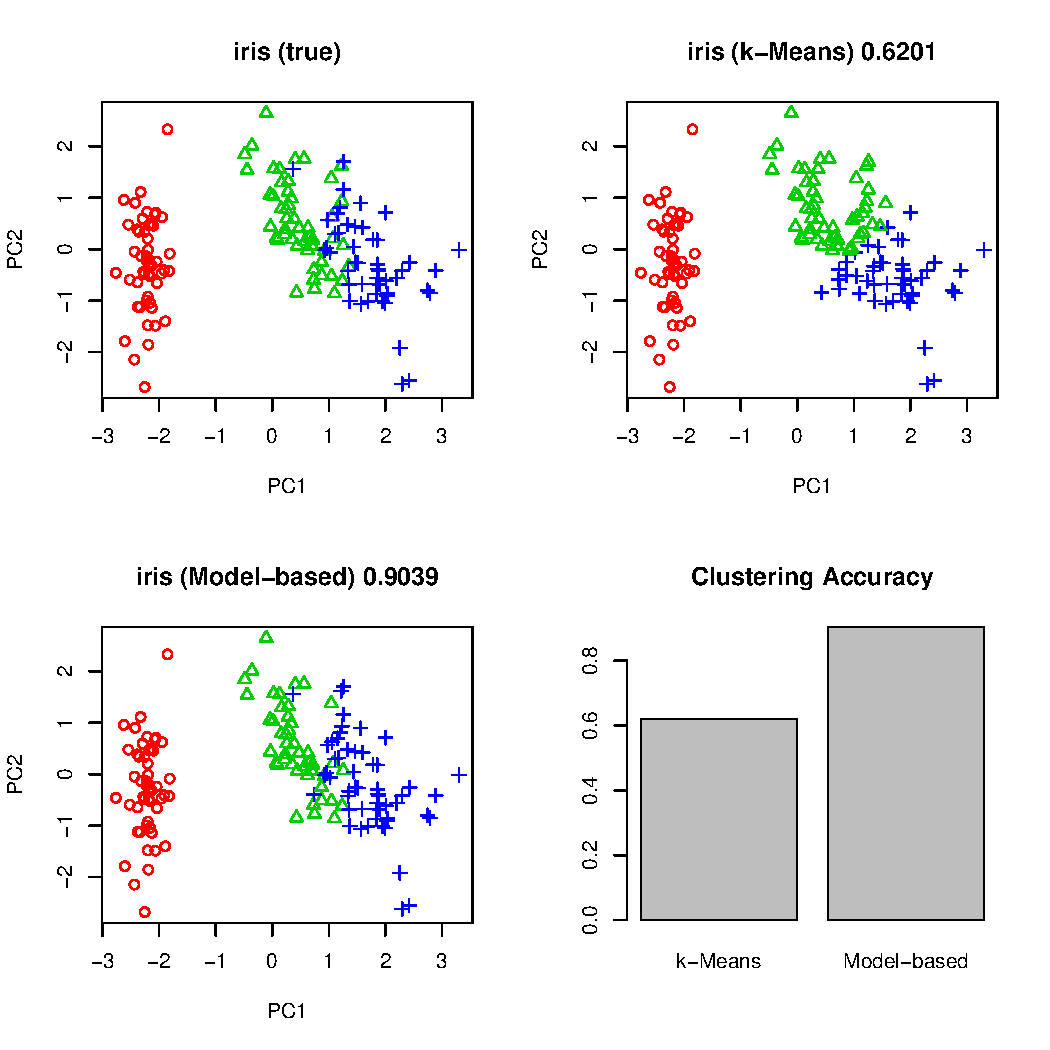
\includegraphics[width=4in]{pbdDEMO-include/pics/serial_plot.pdf}
  \caption{Iris Clustering Plots --- Serial}
  \label{fig:iris_cluster_serial}
\end{figure}
shows the visualization created by this script.








\subsection{{\it Iris} in SPMD Code}

\subsubsection{Code}



\textbf{Step 1:}  PCA\vspace{-.6cm}
\begin{lstlisting}[language=rr]
library(pbdMPI, quiet = TRUE)              # Load library
if(comm.size() != 4)
  comm.stop("4 processors are required.")

### Load data
X <- as.matrix(iris[, -5])                 # Dimension 150 by 4
X.cid <- as.numeric(iris[, 5])             # True id

### Distribute data
jid <- get.jid(nrow(X))
X.spmd <- X[jid,]                          # SPMD row-major format

### Standardize
N <- allreduce(nrow(X.spmd))               # 150
p <- ncol(X.spmd)                          # 4
mu <- allreduce(colSums(X.spmd / N))
X.std <- sweep(X.spmd, 2, mu, FUN = "-")   # Substract mean
std <- sqrt(allreduce(colSums(X.std^2 / (N - 1))))
X.std <- sweep(X.std, 2, std, FUN = "/")   # Divide by SE

### SVD manually in serial
X.tmp <- crossprod(X.std)                  # X'X (local)
X.tmp <- allreduce(X.tmp)
dim(X.tmp) <- c(p, p)
ret <- eigen(X.tmp)                        # X'X = V D^2 V'
d <- sqrt(ret$values)
v <- ret$vectors
u <- X.std %*% v %*% diag(1/d)                        
\end{lstlisting}

\textbf{Step 2:}  Project onto the first two PC's\vspace{-.6cm}
\begin{lstlisting}[language=rr]
### Project on column space of singular vectors
A <- u %*% diag(d)
B <- X.std %*% v                           # A ~ B 
X.prj <- A[, 1:2]                          # Only useful for plot
X.prj <- do.call("rbind", allgather(X.prj))
\end{lstlisting}

\textbf{Step 3:}  Cluster\vspace{-.6cm}
\begin{lstlisting}[language=rr]
### Clustering
library(pmclust, quiet = TRUE)
comm.set.seed(123, diff = TRUE)

X.spmd <- X.std
PARAM.org <- set.global(K = 3)             # Preset storage
.pmclustEnv$CONTROL$debug <- 0             # Disable debug messages
PARAM.org <- initial.center(PARAM.org)     # Initial parameters
PARAM.kms <- kmeans.step(PARAM.org)        # K-means
X.kms.cid <- allgather(.pmclustEnv$CLASS.spmd,
                       unlist = TRUE)

PARAM.org <- set.global(K = 3)             # Preset storage
.pmclustEnv$CONTROL$debug <- 0             # Disable debug messages
PARAM.org <- initial.em(PARAM.org,
                        MU = PARAM.kms$MU) # Initial by K-means
PARAM.mbc1 <- em.step(PARAM.org)           # Model-based clustering
X.mbc1.cid <- allgather(.pmclustEnv$CLASS.spmd,
                        unlist = TRUE)

PARAM.org <- set.global(K = 3, RndEM.iter = 1000)     # Preset storage
.pmclustEnv$CONTROL$debug <- 0             # Disable debug messages
PARAM.org <- initial.RndEM(PARAM.org)      # Initial by Rand-EM
PARAM.mbc2 <- em.step(PARAM.org)           # Model-based clustering
X.mbc2.cid <- allgather(.pmclustEnv$CLASS.spmd,
                        unlist = TRUE)

### Validation
X.kms.adjR <- EMCluster::RRand(X.cid, X.kms.cid)$adjRand
X.mbc1.adjR <- EMCluster::RRand(X.cid, X.mbc1.cid)$adjRand
X.mbc2.adjR <- EMCluster::RRand(X.cid, X.mbc2.cid)$adjRand
comm.print(c(X.kms.adjR, X.mbc1.adjR, X.mbc2.adjR))

### Swap classification id
tmp <- X.kms.cid
X.kms.cid[tmp == 1] <- 2
X.kms.cid[tmp == 2] <- 1
tmp <- X.mbc1.cid
X.mbc1.cid[tmp == 1] <- 2
X.mbc1.cid[tmp == 2] <- 1
\end{lstlisting}

\textbf{Step 4:}  Visualize\vspace{-.6cm}
\begin{lstlisting}[language=rr]
### Display on first 2 components
if(comm.rank() == 0){
  pdf("spmd_plot.pdf")
  
  par(mfrow = c(2, 2))
  plot(X.prj, col = X.cid + 1, pch = X.cid,
       main = "iris (true)", xlab = "PC1", ylab = "PC2")
  plot(X.prj, col = X.kms.cid + 1, pch = X.kms.cid,
       main = paste("iris (kmeans)", sprintf("%.4f", X.kms.adjR)),
       xlab = "PC1", ylab = "PC2")
  plot(X.prj, col = X.mbc1.cid + 1, pch = X.mbc1.cid,
       main = paste("iris (model-based 1)", sprintf("%.4f", X.mbc1.adjR)),
       xlab = "PC1", ylab = "PC2")
  plot(X.prj, col = X.mbc2.cid + 1, pch = X.mbc2.cid,
       main = paste("iris (model-based 2)", sprintf("%.4f", X.mbc2.adjR)),
       xlab = "PC1", ylab = "PC2")

  dev.off()
}

### Finish
finalize()
\end{lstlisting}

\subsubsection{Sample Outputs}
Running this script should produce an ouput that looks something like the following:
\begin{Output}
COMM.RANK = 0
[1] 2.547376e-14 8.076873e-15 4.440892e-14
COMM.RANK = 0
[1] 0.6201352 0.6311581 0.6928082
null device 
          1 
\end{Output}

Finally, figure~\ref{fig:iris_cluster_spmd}
\begin{figure}[h!bt]
  \centering
  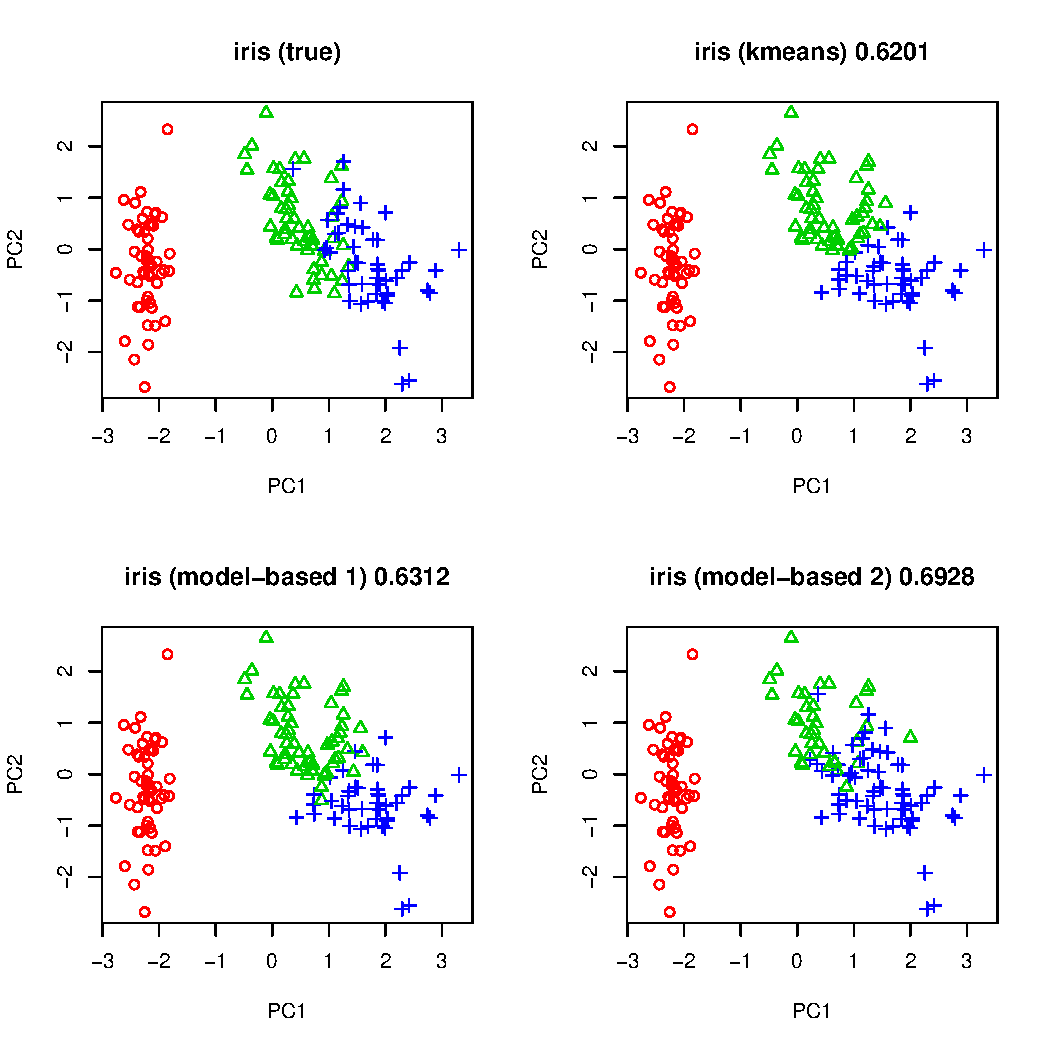
\includegraphics[width=4in]{pbdDEMO-include/pics/spmd_plot.pdf}
  \caption{Iris Clustering Plots --- SPMD}
  \label{fig:iris_cluster_spmd}
\end{figure}
shows the visualization created by this script.













\subsection{{\it Iris} in \code{ddmatrix}\ Code}

\subsubsection{Code}



\textbf{Step 1:}  PCA\vspace{-.6cm}
\begin{lstlisting}[language=rr]
library(pbdDMAT, quiet = TRUE)                        # Load library
init.grid()
if(comm.size() != 4)
  comm.stop("4 processors are required.")

### Load data
X <- as.matrix(iris[, -5])                            # Dimension 150 by 4
X.cid <- as.numeric(iris[, 5])                        # True id

### Convert to ddmatrix
X.dmat <- as.ddmatrix(X)

### Standardized
X.std <- scale(X.dmat)
mu <- as.matrix(colMeans(X.std))
cov <- as.matrix(cov(X.std))
comm.print(mu)
comm.print(cov)

### SVD
X.svd <- svd(X.std)                  
\end{lstlisting}

\textbf{Step 2:}  Project onto the first two PC's\vspace{-.6cm}
\begin{lstlisting}[language=rr]
### Project on column space of singular vectors
A <- X.svd$u %*% diag(X.svd$d, type="ddmatrix")
B <- X.std %*% X.svd$v                                # A ~ B
X.prj <- as.matrix(A[, 1:2])                          # Only useful for plot
\end{lstlisting}

\textbf{Step 3:}  Cluster\vspace{-.6cm}
\begin{lstlisting}[language=rr]
### Clustering
library(pmclust, quiet = TRUE)
comm.set.seed(123, diff = TRUE)

X.dmat <- X.std
PARAM.org <- set.global.dmat(K = 3)                   # Preset storage
.pmclustEnv$CONTROL$debug <- 0                        # Disable debug messages
PARAM.org <- initial.center.dmat(PARAM.org)
PARAM.kms <- kmeans.step.dmat(PARAM.org)              # K-means
X.kms.cid <- as.vector(.pmclustEnv$CLASS.dmat)

### Validation
X.kms.adjR <- EMCluster::RRand(X.cid, X.kms.cid)$adjRand
comm.print(X.kms.adjR)

### Swap classification id
tmp <- X.kms.cid
X.kms.cid[tmp == 1] <- 3
X.kms.cid[tmp == 2] <- 1
X.kms.cid[tmp == 3] <- 2
\end{lstlisting}

\textbf{Step 4:}  Visualize\vspace{-.6cm}
\begin{lstlisting}[language=rr]
### Display on first 2 components
if(comm.rank() == 0){
  pdf("dmat_plot.pdf")
  
  par(mfrow = c(2, 2))
  plot(X.prj, col = X.cid + 1, pch = X.cid,
       main = "iris (true)", xlab = "PC1", ylab = "PC2")
  plot(X.prj, col = X.kms.cid + 1, pch = X.kms.cid,
       main = paste("iris (kmeans)", sprintf("%.4f", X.kms.adjR)),
       xlab = "PC1", ylab = "PC2")
  dev.off()
}

### Finish
finalize()
\end{lstlisting}

\subsubsection{Sample Outputs}
Running this script should produce an ouput that looks something like the following:
\begin{Output}
Using 2x2 for the default grid size

COMM.RANK = 0
              [,1]         [,2]          [,3]         [,4]
[1,] -4.440892e-16 1.990595e-16 -2.428613e-17 2.498002e-16
COMM.RANK = 0
           [,1]       [,2]       [,3]       [,4]
[1,]  1.0000000 -0.1175698  0.8717538  0.8179411
[2,] -0.1175698  1.0000000 -0.4284401 -0.3661259
[3,]  0.8717538 -0.4284401  1.0000000  0.9628654
[4,]  0.8179411 -0.3661259  0.9628654  1.0000000
COMM.RANK = 0
[1] 0.645147

null device 
          1 
\end{Output}

Finally, figure~\ref{fig:iris_cluster_spmd}
\begin{figure}[h!bt]
  \centering
  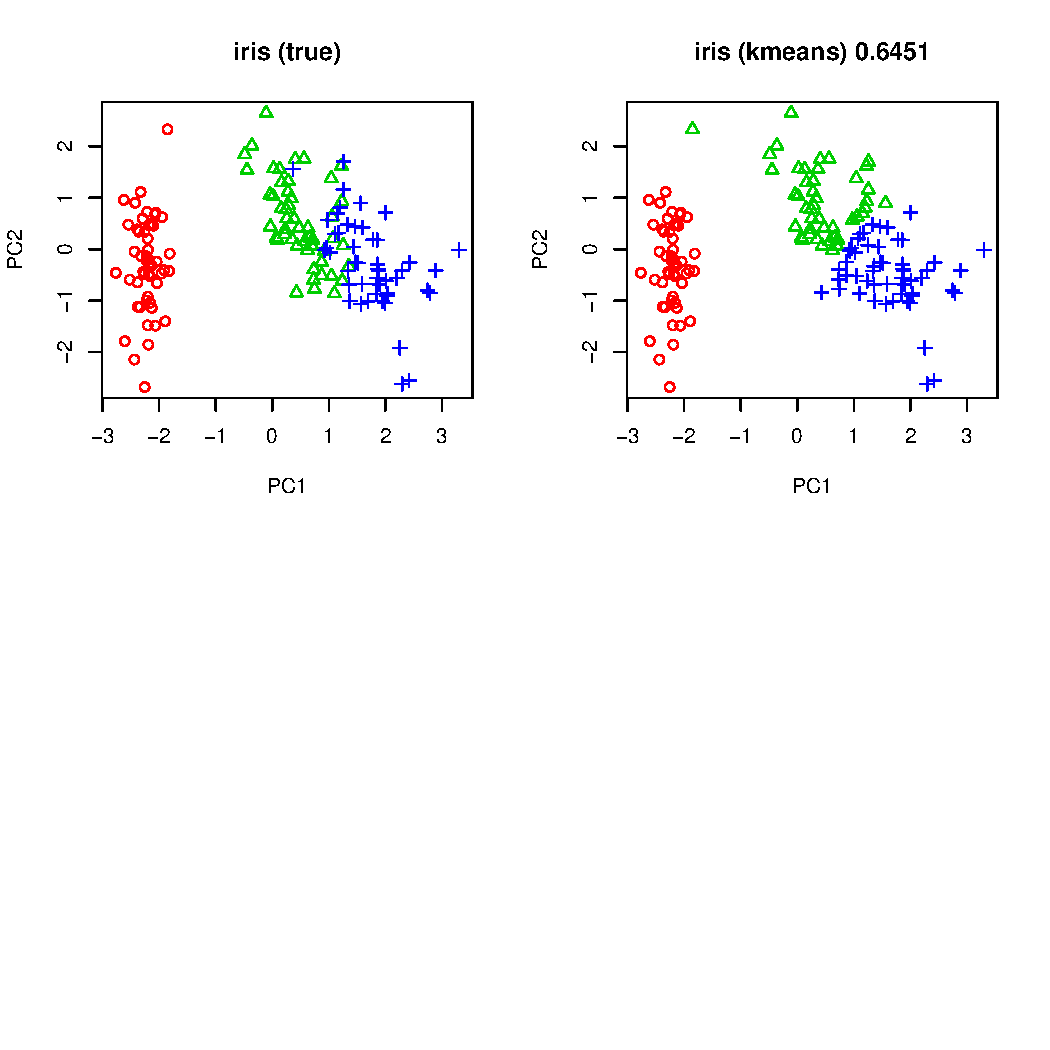
\includegraphics[width=4in]{pbdDEMO-include/pics/dmat_plot.pdf}
  \caption{Iris Clustering Plots --- SPMD}
  \label{fig:iris_cluster_spmd}
\end{figure}
shows the visualization created by this script.




















\section{Exercises}
\label{sec:pmclust_exercise}

\begin{enumerate}[label=\thechapter-\arabic*]
\item

\end{enumerate}

